\documentclass[12pt,a4paper]{report}

% ------ Layout ---------------------------------------------------------------
\usepackage[T1]{fontenc}
\usepackage{lmodern}
\usepackage{microtype}
\usepackage{geometry}
\geometry{
 a4paper,
 left=20mm,
 right=20mm,
 top=20mm,
 bottom=20mm,
}
\setlength{\footskip}{14mm}

% ------ Colours --------------------------------------------------------------
\usepackage[table]{xcolor}
\definecolor{accentblue}{RGB}{0,0,0}

% ------ Graphics -------------------------------------------------------------
\usepackage{graphicx}
\usepackage{float}
\usepackage{eso-pic}
\graphicspath{{./}{screenshots/}}

% ------ Tables ---------------------------------------------------------------
\usepackage{tabularx}
\usepackage{booktabs}
\usepackage{array}
\usepackage{longtable}

% ------ Code listings --------------------------------------------------------
\usepackage{listings}
\lstdefinestyle{mystyle}{
    backgroundcolor=\color{gray!8},
    commentstyle=\color{gray},
    keywordstyle=\bfseries,
    numberstyle=\tiny\color{gray},
    stringstyle=\color{gray},
    basicstyle=\ttfamily\footnotesize,
    breakatwhitespace=false,
    breaklines=true,
    captionpos=b,
    keepspaces=true,
    numbers=left,
    numbersep=5pt,
    showspaces=false,
    showstringspaces=false,
    showtabs=false,
    tabsize=2
}
\lstset{style=mystyle}
\lstdefinestyle{cqlstyle}{style=mystyle}
\lstdefinestyle{bashstyle}{style=mystyle}
\lstdefinestyle{groovystyle}{style=mystyle}

% ------ TikZ -----------------------------------------------------------------
\usepackage{tikz}
\usetikzlibrary{shapes.geometric,arrows.meta,positioning,fit,backgrounds,calc}
\tikzset{
  sysbox/.style={rectangle,rounded corners=4pt,draw=blue!60,fill=blue!8,
    minimum width=2.8cm,minimum height=0.85cm,align=center,
    font=\small,inner sep=4pt},
  dbbox/.style={rectangle,rounded corners=4pt,draw=green!60!black,fill=green!8,
    minimum width=2.8cm,minimum height=0.85cm,align=center,
    font=\small,inner sep=4pt},
  uibox/.style={rectangle,rounded corners=4pt,draw=purple!60,fill=purple!8,
    minimum width=2.8cm,minimum height=0.85cm,align=center,
    font=\small,inner sep=4pt},
  mlbox/.style={rectangle,rounded corners=4pt,draw=orange!70,fill=orange!8,
    minimum width=3.2cm,minimum height=0.85cm,align=center,
    font=\small,inner sep=4pt},
  stagebox/.style={rectangle,rounded corners=4pt,draw=black!60,fill=orange!15,
    minimum width=3.4cm,minimum height=0.8cm,align=center,
    font=\small\bfseries,inner sep=4pt},
  decbox/.style={diamond,draw=black!60,fill=yellow!15,
    minimum width=2.2cm,minimum height=1.2cm,
    align=center,font=\scriptsize,inner sep=2pt},
  startend/.style={ellipse,draw=black!60,fill=gray!15,
    minimum width=2.6cm,minimum height=0.7cm,align=center,font=\small},
  arrow/.style={-Stealth,thick,draw=gray!60},
  darrow/.style={-Stealth,thick,draw=gray!60,dashed},
}

% ------ Misc packages --------------------------------------------------------
\usepackage{enumitem}
\usepackage{caption}
\usepackage{amsmath}
\usepackage{titlesec}
\usepackage{fancyhdr}
\usepackage{setspace}

% ------ Hyperlinks (load last) -----------------------------------------------
\usepackage{hyperref}
\hypersetup{
  colorlinks=true,
  citecolor=accentblue,
  linkcolor=accentblue,
  urlcolor=accentblue
}

% ------ Suppress text overflows gracefully -----------------------------------
\setlength{\emergencystretch}{3em}
% ------ Part numbering A/B ---------------------------------------------------
\renewcommand{\thepart}{\Alph{part}}

\AddToShipoutPictureBG{% 
  \AtPageLowerLeft{% 
    \put(\LenToUnit{10mm},\LenToUnit{10mm}){% 
      \framebox(\LenToUnit{\paperwidth-20mm},\LenToUnit{\paperheight-20mm}){}%
    }%
  }%
}

% ------ Chapter/section typography (Cloud style) -----------------------------
\titleformat{\chapter}[display]
  {\normalfont\centering\bfseries}
  {\chaptertitlename\ \thechapter}{18pt}{\Huge}
  [\vspace{0.8ex}\rule{0.7\textwidth}{0.8pt}]
\titlespacing*{\chapter}{0pt}{18pt}{24pt}

\titleformat{\section}
  {\normalfont\Large\bfseries}
  {\thesection}{1em}{}
\titlespacing*{\section}{0pt}{*2.5}{*1.5}

\titleformat{\subsection}
  {\normalfont\large\bfseries}{\thesubsection}{1em}{}
\titlespacing*{\subsection}{0pt}{*1.5}{*1}

\titleformat{\subsubsection}
  {\normalfont\normalsize\bfseries}{\thesubsubsection}{1em}{}
\titlespacing*{\subsubsection}{0pt}{*1}{*0.5}

% ------ Page style (Cloud style) ---------------------------------------------
\fancypagestyle{plain}{%
  \fancyhf{}
  \fancyfoot[C]{\thepage}
  \renewcommand{\headrulewidth}{0pt}
  \renewcommand{\footrulewidth}{0pt}
}
\fancypagestyle{chapterstyle}{%
  \fancyhf{}
  \fancyfoot[C]{\thepage}
  \renewcommand{\headrulewidth}{0pt}
  \renewcommand{\footrulewidth}{0pt}
}

\newif\ifshowimages
\showimagestrue

\newcommand{\myimage}[2]{%
  \ifshowimages
    \IfFileExists{#2}{\includegraphics[width=#1]{#2}}{\fbox{\ttfamily\detokenize{#2}}}
  \else
    \fbox{\ttfamily\detokenize{#2}}
  \fi
}

% ------ Screenshot placeholder -----------------------------------------------
\newcommand{\screenshotfig}[3]{%
  \begin{figure}[H]
    \centering
    \fbox{\parbox{0.80\linewidth}{\centering
      \vspace{1.0cm}
      {\large\textit{[Screenshot: #2]}}\\[0.5cm]
      {\small\nolinkurl{screenshots/#1}}%
      \vspace{1.0cm}
    }}%
    \caption{#2}%
    \label{#3}%
  \end{figure}%
}
% =============================================================================
\begin{document}
\linespread{1.39}\selectfont
\pagestyle{plain}
\onehalfspacing
\pagenumbering{gobble}
% =============================================================================

% ---- TITLE PAGE -------------------------------------------------------------
\begin{titlepage}
\begin{center}
\textsc{\Large\textcolor{accentblue}{B.M.S.\ COLLEGE OF ENGINEERING}}\\[0.1cm]
\textsc{(Autonomous College under VTU)}\\[0.1cm]
\textsc{Bull Temple Road, Basavangudi, Bangalore -- 560019}\\[0.5cm]

\myimage{0.50\linewidth}{logo.png}\\[0.4cm]

\textbf{\Large DEVOPS LAB REPORT}\\[0.5cm]
\textbf{BACHELOR OF ENGINEERING}\\
\textit{in}\\
\textbf{Computer Science \& Engineering -- Data Science}\\[0.5cm]

\textit{Submitted by}\\[0.3cm]
\begin{tabular}{ll}
  \textbf{H Sampreeth Bhat}  & \textbf{1BM23CD020} \\
  \textbf{R V Abhishek}      & \textbf{1BM23CD047} \\
  \textbf{Ullas N}           & \textbf{1BM23CD067} \\
\end{tabular}\\[0.7cm]

\textbf{Under the Guidance of}\\[0.2cm]
\textbf{Sandhya G}\\[0.9cm]

\textbf{Department of CSE -- Data Science}\\
\textbf{B.M.S.\ College of Engineering}\\[0.4cm]
\textbf{AY 2025--2026}
\end{center}
\end{titlepage}
\pagenumbering{roman}
\setcounter{page}{1}

% ---- CERTIFICATE ------------------------------------------------------------
\newpage
\thispagestyle{plain}
\begin{center}
  \textbf{\Large CERTIFICATE}
\end{center}
\vspace{0.5cm}

This is to certify that the DevOps Lab report titled
\textit{``Real-Time Network Intrusion Detection System using NoSQL Databases
and CI/CD Pipeline''} submitted by \textbf{Ullas N (1BM23CD067)},
\textbf{H Sampreeth Bhat (1BM23CD020)}, and \textbf{R V Abhishek (1BM23CD047)} is a
bonafide record of work carried out under my supervision during the academic
year 2025--2026, in partial fulfilment of the requirements for the award of
the degree of Bachelor of Engineering in Computer Science \& Engineering
(Data Science) at B.M.S.\ College of Engineering, Bangalore.

\vspace{1cm}
\begin{center}
  \begin{tabular}{ccc}
    \toprule
    \textbf{Sl.\ No.} & \textbf{Name} & \textbf{USN} \\
    \midrule
    1 & Ullas N & 1BM23CD067 \\
    2 & H Sampreeth Bhat & 1BM23CD020 \\
    3 & R V Abhishek & 1BM23CD047 \\
    \bottomrule
  \end{tabular}
\end{center}
\vspace{1.5cm}
\noindent\textbf{Guide: Sandhya G}\hfill\textbf{HOD}
\vfill
\noindent\textbf{Date:} 24 April 2026

% ---- DECLARATION ------------------------------------------------------------
\newpage
\thispagestyle{plain}
\begin{center}
  \textbf{\Large DECLARATION}
\end{center}
\vspace{0.5cm}

We, \textbf{Ullas N (1BM23CD067)}, \textbf{H Sampreeth Bhat (1BM23CD020)},
and \textbf{R V Abhishek (1BM23CD047)}, hereby declare that this DevOps Lab
report titled \textit{``Real-Time Network Intrusion Detection System using
NoSQL Databases and CI/CD Pipeline''} is a bonafide record of work carried
out by us under the guidance of \textbf{Sandhya G}.  This work has not been
submitted elsewhere for any degree or examination.

\vspace{1.5cm}
\begin{center}
  \begin{tabular}{ccc}
    \toprule
    \textbf{Sl.\ No.} & \textbf{Name} & \textbf{USN} \\
    \midrule
    1 & Ullas N & 1BM23CD067 \\
    2 & H Sampreeth Bhat & 1BM23CD020 \\
    3 & R V Abhishek & 1BM23CD047 \\
    \bottomrule
  \end{tabular}
\end{center}
\vspace{1.5cm}
\noindent\textbf{Signature of Students}\hfill\textbf{Signature of Guide}
\vfill
\noindent\textbf{Date:} 24 April 2026

% ---- TABLE OF CONTENTS ------------------------------------------------------
\tableofcontents
\newpage
\listoffigures
\newpage
\listoftables
\newpage

% ---- ABSTRACT ---------------------------------------------------------------
\thispagestyle{plain}
\begin{center}
  \textbf{\Large ABSTRACT}
\end{center}
\vspace{0.5cm}

This report presents a real-time Network Intrusion Detection System (NIDS)
that combines streaming analytics, machine learning inference, and NoSQL data
management in a production-style DevOps workflow. The system ingests
UNSW-NB15 traffic records through Apache Kafka, performs two-stage inference
using Gradient Boosted Trees (binary attack detection) and Random Forest
(attack-type classification), and stores outputs in a Cassandra + Redis dual
database architecture for durable persistence and low-latency dashboard reads.

The implementation is integrated with a Jenkins-driven CI/CD pipeline that
automates linting, testing, image builds, and branch-gated deployment using
Docker Compose. The design demonstrates how model-serving, stream processing,
NoSQL storage, and deployment automation can be combined into a reproducible
and scalable cybersecurity analytics platform suitable for academic and
industry-aligned DevOps practice.
\newpage

% #############################################################################
\pagenumbering{arabic}
\part{Next Gen Databases (NGD)}
This part explains the storage architecture of the NIDS platform, including
the rationale for selecting Cassandra and Redis, schema design decisions,
query patterns, and performance-oriented data operations.
% #############################################################################

% =============================================================================
\chapter{Introduction}
% =============================================================================

\section{Project Title}
\textbf{Real-Time Network Intrusion Detection System (NIDS) using NoSQL
Databases and Machine Learning.}

\section{Objective}
The objective of this project is to design and implement a real-time network
intrusion detection system that:
\begin{itemize}
  \item Ingests high-velocity network traffic records streamed through
        Apache Kafka.
  \item Performs \textbf{two-stage machine learning inference}:
        \begin{enumerate}
          \item \textbf{Binary classification} (Gradient Boosted Trees, GBT)
                to determine whether each record is \textit{Normal} or an
                \textit{Attack}.
          \item \textbf{Multiclass classification} (Random Forest) to identify
                the specific attack category among nine types.
        \end{enumerate}
  \item Persists every intrusion alert in \textbf{Apache Cassandra} for
        durable, fault-tolerant long-term storage.
  \item Caches live alerts in \textbf{Redis} for sub-millisecond dashboard
        reads and real-time pub/sub notifications.
  \item Exposes a \textbf{Flask-based web dashboard} with live severity
        gauges, filterable alert tables, and analytics charts for security
        analysts.
\end{itemize}

\section{Problem Statement / Use Case}

\subsection{Problem Statement}
Modern enterprise and campus networks generate millions of traffic records per
minute.  Traditional signature-based Intrusion Detection Systems (IDS)
maintain a fixed list of known attack signatures and fail against novel or
zero-day exploits.  Relational database management systems (RDBMS) are
ill-suited for this streaming workload because:
\begin{itemize}
  \item \textbf{Schema rigidity:} Adding new protocol fields requires
        \texttt{ALTER TABLE}, causing downtime.
  \item \textbf{Write bottlenecks:} SQL \texttt{INSERT} operations acquire
        row-level locks and incur B-tree index overhead at high insert rates.
  \item \textbf{No horizontal scaling:} RDBMS instances scale vertically
        (larger machines), which is expensive and finite.
  \item \textbf{JOIN overhead:} Analytical queries joining alerts with session
        metadata become prohibitively slow at millions of rows.
\end{itemize}

\subsection{Use Case}
A university or enterprise Network Operations Centre (NOC) uses this system to:
\begin{enumerate}
  \item Continuously stream network traffic through the Kafka pipeline at up
        to 100 records per second (scalable to millions).
  \item Automatically flag and classify suspicious traffic in real time via
        trained ML models with no human intervention.
  \item Query historical alerts by session, time range, or attack category
        through the Flask REST API and dashboard.
  \item Receive instant live notifications the moment a high-severity threat
    (DoS, Exploits, Shellcode, Backdoor) is detected via Redis pub/sub.
\end{enumerate}

The system uses the \textbf{UNSW-NB15 dataset} from the University of New South
  Wales Canberra---a benchmark network security dataset with 2.5 million raw
  traffic records and a standard train/test split of 175,341 / 82,332 records
  used for model training and evaluation, with 42 feature columns and 9
  distinct attack categories.

\begin{figure}[H]
\centering
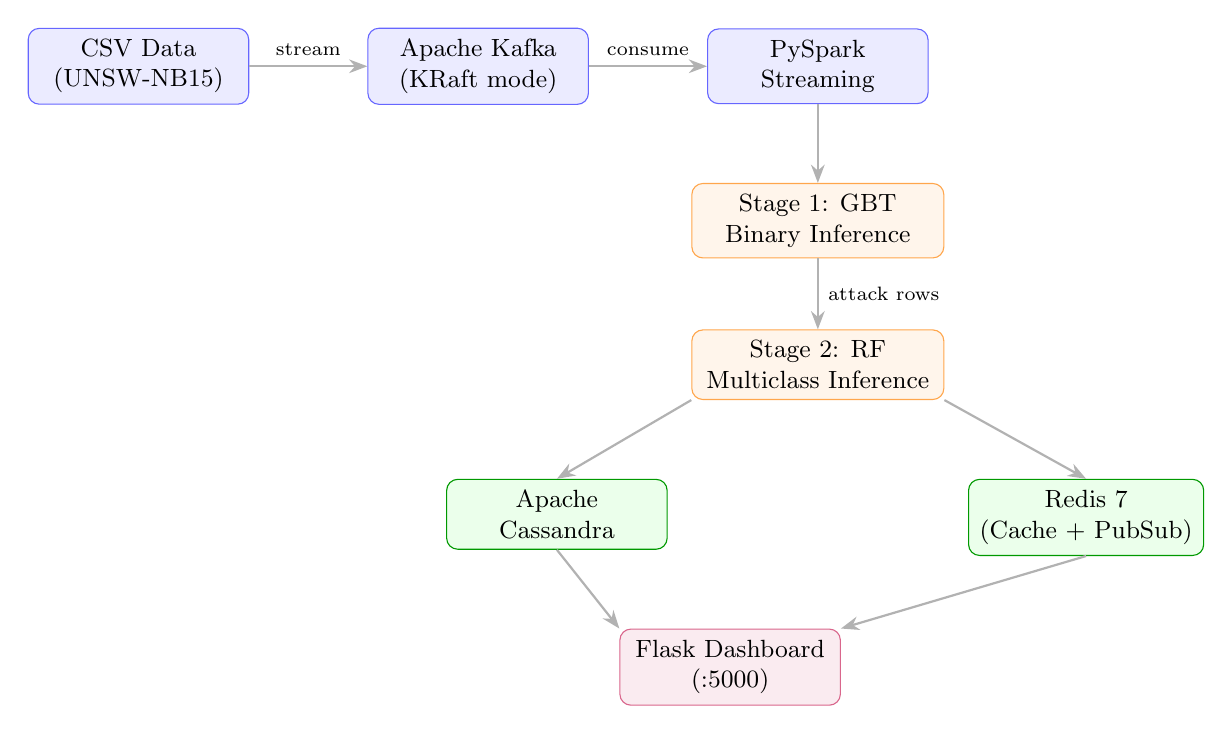
\begin{tikzpicture}[node distance=1.0cm and 1.5cm]
  \node[sysbox] (csv)   {CSV Data\\(UNSW-NB15)};
  \node[sysbox, right=of csv]    (kafka)  {Apache Kafka\\(KRaft mode)};
  \node[sysbox, right=of kafka]  (spark)  {PySpark\\Streaming};
  \node[mlbox,  below=1.0cm of spark] (gbt) {Stage 1: GBT\\Binary Inference};
  \node[mlbox,  below=0.9cm of gbt]   (rf)  {Stage 2: RF\\Multiclass Inference};
  \node[dbbox,  below left=1.0cm and 0.3cm of rf]  (cass)  {Apache\\Cassandra};
  \node[dbbox,  below right=1.0cm and 0.3cm of rf] (redis) {Redis 7\\(Cache + PubSub)};
  \node[uibox,  below=1.0cm of cass, xshift=2.2cm] (flask) {Flask Dashboard\\(:5000)};
  \draw[arrow] (csv)   -- node[above,font=\scriptsize]{stream} (kafka);
  \draw[arrow] (kafka) -- node[above,font=\scriptsize]{consume} (spark);
  \draw[arrow] (spark) -- (gbt);
  \draw[arrow] (gbt)   -- node[right,font=\scriptsize]{attack rows} (rf);
  \draw[arrow] (rf.south west) -- (cass.north);
  \draw[arrow] (rf.south east) -- (redis.north);
  \draw[arrow] (cass.south)  -- (flask.north west);
  \draw[arrow] (redis.south) -- (flask.north east);
\end{tikzpicture}
\caption{High-level system architecture of the Real-Time NIDS}
\label{fig:architecture}
\end{figure}
\begin{center}

\begin{tikzpicture}[baseline]
  \node[sysbox, minimum width=0.9cm, minimum height=0.35cm, inner sep=1pt] at (0,0) {};
  \node[anchor=west,font=\scriptsize] at (0.55,0) {System Components};
  \node[dbbox, minimum width=0.9cm, minimum height=0.35cm, inner sep=1pt] at (4.1,0) {};
  \node[anchor=west,font=\scriptsize] at (4.65,0) {Databases};
  \node[uibox, minimum width=0.9cm, minimum height=0.35cm, inner sep=1pt] at (7.3,0) {};
  \node[anchor=west,font=\scriptsize] at (7.85,0) {Dashboard/UI};
  \node[mlbox, minimum width=0.9cm, minimum height=0.35cm, inner sep=1pt] at (10.6,0) {};
  \node[anchor=west,font=\scriptsize] at (11.15,0) {ML Inference};
\end{tikzpicture}
\end{center}

% =============================================================================
\chapter{Selection and Justification of NoSQL Database}
% =============================================================================

\section{Types of NoSQL Databases Used}
This project employs \textbf{two complementary NoSQL databases}, each serving
a distinct role:

\begin{enumerate}
  \item \textbf{Apache Cassandra 4.1}---a \textbf{Wide-Column Store} used for
        durable, partitioned alert persistence (source of truth).
  \item \textbf{Redis 7}---a \textbf{Key-Value Store} (with list, hash, and
        pub/sub support) used for in-memory caching and real-time event
        delivery (speed layer).
\end{enumerate}

\section{Reason for Selection}

\subsection{Apache Cassandra}
\begin{itemize}
  \item Designed for \textbf{high-write-throughput}: uses an LSM-tree
        (Log-Structured Merge-tree) storage engine with no row locks---every
        write is a sequential append.
  \item \textbf{Partition key model} distributes session-specific alert data
        across cluster nodes automatically via consistent hashing.
  \item \textbf{Clustering key} stores rows pre-sorted in
        reverse-chronological order on disk, making ``latest $N$ alerts''
        queries free (no sort step at query time).
  \item \textbf{Linear horizontal scalability}: adding nodes increases
        throughput proportionally without re-sharding.
  \item CQL (Cassandra Query Language) provides a familiar SQL-like syntax
        for DDL and DML operations.
\end{itemize}

\subsection{Redis}
\begin{itemize}
  \item In-memory data structure store guarantees
        \textbf{sub-millisecond read latency}---essential for a dashboard
        that auto-refreshes every 5 seconds.
  \item The \textbf{LPUSH\,/\,LRANGE} list primitives maintain an ordered
        recent-alerts cache without application-level sorting.
  \item The built-in \textbf{pub/sub channel}
        (\texttt{alert\_notifications}) allows the Spark pipeline to push
        live events to subscribed clients without polling.
  \item Acts as a \textbf{speed layer}: absorbs all dashboard read traffic,
        protecting Cassandra from repeated identical queries.
  \item Configurable \textbf{key TTL} automatically evicts stale session
        caches, preventing unbounded memory growth.
\end{itemize}

\section{Why It Suits the Use Case}
The NIDS use case has two conflicting requirements:
\begin{itemize}
  \item \textbf{Fast writes:} Spark commits up to 100 alert records per
        30-second micro-batch continuously.
  \item \textbf{Fast reads:} The live dashboard must serve alert feeds with
        latency below 50 ms.
\end{itemize}
No single database handles both optimally.  The
\textbf{dual-database design} resolves this tension:
\begin{itemize}
  \item Cassandra absorbs all writes as the \textit{source of truth}.
  \item Redis mirrors recent writes as a \textit{read cache}, refreshed by
        each Spark micro-batch and invalidated by TTL after one hour.
\end{itemize}

\section{Brief Comparison with Relational Database}
\begin{table}[H]
  \centering
  \caption{NoSQL vs.\ RDBMS comparison for the NIDS use case}
  \label{tab:nosql-vs-rdbms}
  \rowcolors{2}{blue!4}{white}
  \begin{tabularx}{\textwidth}{lXXX}
    \toprule
    \textbf{Criterion} & \textbf{RDBMS (PostgreSQL)} &
    \textbf{Cassandra} & \textbf{Redis} \\
    \midrule
    Schema flexibility  & Fixed; \texttt{ALTER TABLE} needed &
    Flexible; add columns freely & Schema-free key-value \\
    Write throughput    & Medium (WAL, row locks) &
    Very high (LSM-tree, no locks) & Extremely high (RAM) \\
    Read latency        & Low--medium (with index) &
    Low (partition + cluster key) & Sub-millisecond \\
    Horizontal scaling  & Difficult (manual sharding) &
    Native (token ring) & Cluster mode \\
    Persistence         & Durable (WAL) &
    Durable (commit log + SSTables) & Optional (AOF/RDB) \\
    Query language      & Full SQL with JOINs &
    CQL (no JOINs) & Commands (GET, LRANGE, \ldots) \\
    Best fit            & Not ideal for NIDS &
    Alert archival & Live dashboard feed \\
    \bottomrule
  \end{tabularx}
\end{table}

% =============================================================================
\chapter{Data Model and Schema Design}
% =============================================================================

\section{Data Model Description}
The data model spans two storage tiers.

\subsection{Apache Cassandra -- Wide-Column Store}
The Cassandra keyspace \texttt{nids} contains two tables:
\begin{itemize}
  \item \textbf{\texttt{nids.alerts}}---stores every intrusion alert detected
        by the ML pipeline.  Partitioned by \texttt{session\_id} and
        clustered by \texttt{alert\_time DESC}.
  \item \textbf{\texttt{nids.sessions}}---stores metadata for each streaming
        session (dataset name, creation timestamp).
\end{itemize}

\subsection{Redis -- Key-Value Store}
Redis maintains five key patterns:
\begin{itemize}
  \item \texttt{nids:alerts:\{session\_id\}}---ordered list of JSON-encoded
        alert objects, newest first (capped at 1\,000 entries).
  \item \texttt{nids:sessions}---list of all known session IDs.
  \item \texttt{nids:stats:\{session\_id\}}---JSON blob of pre-aggregated
        counts by severity and attack type.
  \item \texttt{nids:timeline:\{session\_id\}}---JSON array of time-bucketed
        alert counts for the analytics chart.
  \item \texttt{alert\_notifications}---pub/sub channel published by the
        Spark pipeline for real-time event delivery.
\end{itemize}

\section{Structure / Attributes}

\subsection{Cassandra nids.alerts Table}
\rowcolors{2}{blue!4}{white}
\begin{longtable}{llp{6cm}}
  \caption{Column definitions for \texttt{nids.alerts}}
  \label{tab:alerts-cols} \\
  \toprule
  \textbf{Column} & \textbf{Type} & \textbf{Description} \\
  \midrule\endfirsthead
  \toprule
  \textbf{Column} & \textbf{Type} & \textbf{Description} \\
  \midrule\endhead
  \texttt{session\_id}      & text   & \textbf{Partition key} --- groups all
    alerts for one session on the same Cassandra node \\
  \texttt{alert\_time}      & text   & \textbf{Clustering key (DESC)} ---
    ISO~8601 timestamp; rows stored newest-first within the partition \\
  \texttt{alert\_id}        & text   & \textbf{Clustering key (ASC)} ---
    UUID ensuring uniqueness when two alerts share the same timestamp \\
  \texttt{attack\_type}     & text   & Human-readable attack category
    (e.g.\ DoS, Exploits, Fuzzers) \\
  \texttt{severity}         & text   & Severity tier: \textit{high} /
    \textit{medium} / \textit{low} / \textit{info} \\
  \texttt{src\_ip}          & text   & Source IP address \\
  \texttt{dst\_ip}          & text   & Destination IP address \\
  \texttt{src\_port}        & int    & Source port number \\
  \texttt{dst\_port}        & int    & Destination port number \\
  \texttt{protocol}         & text   & Network protocol (tcp / udp / other)\\
  \texttt{binary\_prediction}  & int    & GBT output: 0 = Normal, 1 = Attack\\
  \texttt{binary\_probability} & double & GBT confidence score (0.0--1.0) \\
  \texttt{attack\_confidence}  & double & RF confidence for the predicted
    attack type (0.0--1.0) \\
  \texttt{sbytes}           & int    & Source-to-destination bytes \\
  \texttt{dbytes}           & int    & Destination-to-source bytes \\
  \texttt{rate}             & double & Connection rate (packets/second) \\
  \bottomrule
\end{longtable}

\subsection{Cassandra nids.sessions Table}
\begin{table}[H]
  \centering
  \caption{Column definitions for \texttt{nids.sessions}}
  \label{tab:sessions-cols}
  \rowcolors{2}{blue!4}{white}
  \begin{tabular}{llp{7cm}}
    \toprule
    \textbf{Column}   & \textbf{Type} & \textbf{Description} \\
    \midrule
    \texttt{session\_id}  & text & \textbf{Primary key} --- UUID for the
      streaming session \\
    \texttt{dataset}      & text & Dataset name (e.g.\ ``unsw'') \\
    \texttt{created\_at}  & text & ISO~8601 start timestamp \\
    \bottomrule
  \end{tabular}
\end{table}

\subsection{Redis Key Patterns}
\begin{table}[H]
  \centering
  \caption{Redis key patterns and data types}
  \label{tab:redis-keys}
  \rowcolors{2}{blue!4}{white}
  \begin{tabularx}{\textwidth}{llX}
    \toprule
    \textbf{Key Pattern}                  & \textbf{Type} & \textbf{Contents} \\
    \midrule
    \texttt{nids:alerts:\{sid\}}         & List & JSON alert objects, newest
      first; capped at 1\,000 \\
    \texttt{nids:sessions}               & List & All session IDs \\
    \texttt{nids:stats:\{sid\}}          & String (JSON) & Aggregated counts
      by severity and attack type \\
    \texttt{nids:timeline:\{sid\}}       & String (JSON) & Hourly bucketed
      alert counts for analytics \\
    \texttt{alert\_notifications}        & Pub/Sub & Real-time event stream
      from Spark pipeline \\
    \bottomrule
  \end{tabularx}
\end{table}

\section{Relationships / Organisation}
The two Cassandra tables are logically linked via \texttt{session\_id},
which acts as an application-level foreign-key equivalent.  Cassandra does not
support cross-partition JOINs; instead the application queries
\texttt{nids.sessions} first to validate the session, then queries
\texttt{nids.alerts} with the same \texttt{session\_id} as the partition key.

Redis mirrors this organisation: every session-scoped Redis key embeds the
same \texttt{session\_id} token, keeping the cache and database logically
aligned without requiring cross-database JOINs.

\section{Schema Diagram}

\begin{figure}[H]
\centering
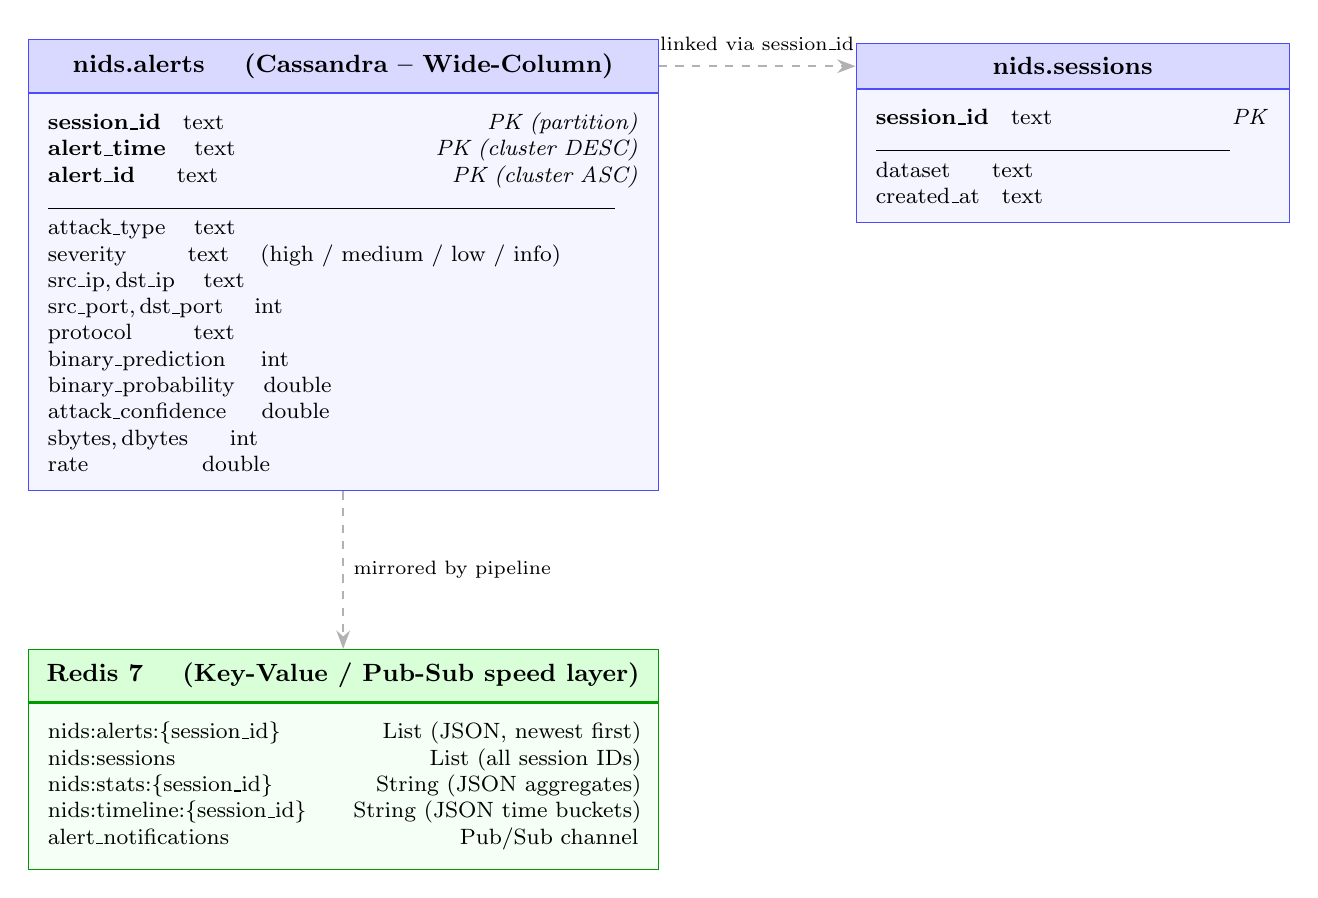
\begin{tikzpicture}

  % nids.alerts header
  \node[draw=blue!70,fill=blue!15,font=\small\bfseries,
        inner sep=5pt,text centered,minimum width=8cm] (ahdr) at (0,0)
    {nids.alerts \quad (Cassandra -- Wide-Column)};

  % nids.alerts body
  \node[draw=blue!70,fill=blue!4,font=\footnotesize,
        align=left,inner sep=7pt,below=0cm of ahdr,
        minimum width=8cm,text width=7.5cm] (abody)
  {
    \textbf{session\_id} \; text \hfill \textit{PK (partition)}\\
    \textbf{alert\_time} \;\; text \hfill \textit{PK (cluster DESC)}\\
    \textbf{alert\_id} \;\;\;\; text \hfill \textit{PK (cluster ASC)}\\
    \rule{7.2cm}{0.3pt}\\
    attack\_type \;\; text\\
    severity \;\;\;\;\;\;\; text \quad (high / medium / low / info)\\
    src\_ip,\,dst\_ip \;\; text\\
    src\_port,\,dst\_port \quad int\\
    protocol \;\;\;\;\;\;\; text\\
    binary\_prediction \;\;\; int\\
    binary\_probability \;\; double\\
    attack\_confidence \;\;\; double\\
    sbytes,\,dbytes \;\;\;\; int\\
    rate \;\;\;\;\;\;\;\;\;\;\;\;\;\;\; double
  };

  % nids.sessions header
  \node[draw=blue!70,fill=blue!15,font=\small\bfseries,
        inner sep=5pt,text centered,minimum width=5.5cm,
        right=2.5cm of ahdr] (shdr)
    {nids.sessions};

  % nids.sessions body
  \node[draw=blue!70,fill=blue!4,font=\footnotesize,
        align=left,inner sep=7pt,below=0cm of shdr,
        minimum width=5.5cm,text width=5.0cm] (sbody)
  {
    \textbf{session\_id} \; text \hfill \textit{PK}\\
    \rule{4.5cm}{0.3pt}\\
    dataset \;\;\;\; text\\
    created\_at \; text
  };

  % Redis header
  \node[draw=green!60!black,fill=green!15,font=\small\bfseries,
        inner sep=5pt,text centered,minimum width=8cm,
        below=2.0cm of abody] (rhdr)
    {Redis 7 \quad (Key-Value / Pub-Sub speed layer)};

  % Redis body
  \node[draw=green!60!black,fill=green!4,font=\footnotesize,
        align=left,inner sep=7pt,below=0cm of rhdr,
        minimum width=8cm,text width=7.5cm] (rbody)
  {
    nids:alerts:\{session\_id\} \hfill List (JSON, newest first)\\
    nids:sessions \hfill List (all session IDs)\\
    nids:stats:\{session\_id\} \hfill String (JSON aggregates)\\
    nids:timeline:\{session\_id\} \hfill String (JSON time buckets)\\
    alert\_notifications \hfill Pub/Sub channel
  };

  % Relationship arrows
  \draw[darrow] (ahdr.east) -- node[above,font=\scriptsize,yshift=2pt]
    {linked via session\_id} (shdr.west);
  \draw[darrow] (abody.south) -- node[right,font=\scriptsize]
    {mirrored by pipeline} (rhdr.north);

\end{tikzpicture}
\caption{Cassandra and Redis data model for the NIDS project}
\label{fig:schema-diagram}
\end{figure}

% =============================================================================
\chapter{Implementation and Query Processing}
% =============================================================================

\section{Structure Creation}

\subsection{Creating the Keyspace}
The Cassandra keyspace \texttt{nids} is the top-level namespace, analogous to
a database in an RDBMS.

\begin{lstlisting}[style=cqlstyle,
  caption={CQL: Create the nids keyspace},
  label={lst:keyspace}]
CREATE KEYSPACE IF NOT EXISTS nids
WITH replication = {
    'class': 'SimpleStrategy',
    'replication_factor': 1
};
\end{lstlisting}

\textbf{What this query does:}  Creates the \texttt{nids} keyspace if it does
not already exist.  \texttt{IF NOT EXISTS} makes it idempotent---safe to
execute on every application restart.  \texttt{SimpleStrategy} with
\texttt{replication\_factor~=~1} is used for single-node development; in a
production cluster this would be \texttt{NetworkTopologyStrategy} with
\texttt{replication\_factor~=~3} to survive two-node failures.

\textbf{Why it is used:}  All Cassandra tables must belong to a keyspace.  The
replication strategy and factor are the most important tuning parameters---they
determine how many copies of each partition exist across the cluster.

\subsection{Creating the Alerts Table}
\begin{lstlisting}[style=cqlstyle,
  caption={CQL: Create the nids.alerts table},
  label={lst:alerts-ddl}]
CREATE TABLE IF NOT EXISTS nids.alerts (
    session_id          text,
    alert_time          text,
    alert_id            text,
    attack_type         text,
    severity            text,
    src_ip              text,
    dst_ip              text,
    src_port            int,
    dst_port            int,
    protocol            text,
    binary_prediction   int,
    binary_probability  double,
    attack_confidence   double,
    sbytes              int,
    dbytes              int,
    rate                double,
    PRIMARY KEY (session_id, alert_time, alert_id)
) WITH CLUSTERING ORDER BY (alert_time DESC, alert_id ASC);
\end{lstlisting}

\textbf{What this query does:}  Creates the main alerts table with a
\textbf{composite primary key}:
\begin{itemize}
  \item \texttt{session\_id} (partition key)---all alerts for a session land
        on the same Cassandra node (or replica set), enabling single-partition
        queries.
  \item \texttt{alert\_time DESC} (first clustering column)---rows within a
        partition are physically sorted newest-first, so
        \texttt{SELECT~\ldots~LIMIT~100} always returns the 100 most recent
        alerts without a full scan.
  \item \texttt{alert\_id ASC} (second clustering column)---guarantees
        uniqueness when two alerts share the same millisecond timestamp.
\end{itemize}

\textbf{Why it is used:}  Cassandra's read performance is determined entirely
by the primary key design.  By designing the key to match the dominant query
pattern (``give me the latest $N$ alerts for session $X$''), that query
executes in O(1) partition lookups regardless of total keyspace size.

\subsection{Creating the Sessions Table}
\begin{lstlisting}[style=cqlstyle,
  caption={CQL: Create the nids.sessions table},
  label={lst:sessions-ddl}]
CREATE TABLE IF NOT EXISTS nids.sessions (
    session_id  text PRIMARY KEY,
    dataset     text,
    created_at  text
);
\end{lstlisting}

\textbf{What this query does:}  A simple lookup table with \texttt{session\_id}
as the sole primary key.  Each row records when a streaming session started
and which dataset it processed.

\textbf{Why it is used:}  The Settings page of the dashboard calls
\texttt{/api/sessions} to display a history of all streaming sessions.
Querying by a single primary key is a constant-time Cassandra lookup.

% ----------------------------------------------------------------------------
\section{Data Insertion and Update}

\subsection{Inserting Alert Records into Cassandra}
Every time the Spark pipeline processes a micro-batch, it inserts one row per
detected attack into Cassandra via the following prepared statement.

\begin{lstlisting}[style=cqlstyle,
  caption={CQL: Insert one alert record (prepared statement)},
  label={lst:insert-alert}]
INSERT INTO nids.alerts (
    session_id, alert_time, alert_id,
    attack_type, severity,
    src_ip, dst_ip, src_port, dst_port, protocol,
    binary_prediction, binary_probability,
    attack_confidence,
    sbytes, dbytes, rate
) VALUES (?, ?, ?, ?, ?, ?, ?, ?, ?, ?, ?, ?, ?, ?, ?, ?);
\end{lstlisting}

\textbf{What this query does:}  Writes all 16 fields of an alert in a single
CQL operation using a prepared statement (parameterised with \texttt{?}).
Prepared statements are compiled once by the \texttt{cassandra-driver} Python
library and reused for every subsequent insertion, reducing driver-to-coordinator
round-trip overhead.

\textbf{Why it is used:}  Cassandra's LSM-tree engine makes inserts always fast
(no row locking, no index rebuild on write).  In the Spark pipeline, this
insert is called within a \texttt{foreachBatch} writer so each micro-batch
commits all its alert rows in one driver session, amortising connection setup
cost.

\subsection{Registering a New Session}
\begin{lstlisting}[style=cqlstyle,
  caption={CQL: Register a new streaming session},
  label={lst:insert-session}]
INSERT INTO nids.sessions (session_id, dataset, created_at)
VALUES (?, ?, ?);
\end{lstlisting}

\textbf{What this query does:}  Records the session UUID, dataset name
(e.g.\ ``unsw''), and start timestamp when the pipeline begins streaming.
This is called once at pipeline startup via \texttt{AlertStorage.register\_session()}.

\subsection{Caching Alerts in Redis}
In parallel with the Cassandra write, the pipeline caches the serialised alert
in Redis:

\begin{lstlisting}[style=bashstyle,
  caption={Redis commands: push alert to cache and manage TTL},
  label={lst:redis-push}]
LPUSH  nids:alerts:{session_id}  "<json_alert_string>"
LTRIM  nids:alerts:{session_id}  0  999    # keep newest 1 000 entries
EXPIRE nids:alerts:{session_id}  3600      # auto-evict after 1 hour
\end{lstlisting}

\textbf{What these commands do:}
\begin{itemize}
  \item \texttt{LPUSH} prepends the new alert to the head of the list (newest
        first), mirroring the Cassandra clustering order.
  \item \texttt{LTRIM} caps the list at 1\,000 entries to prevent unbounded
        memory growth in long-running sessions.
  \item \texttt{EXPIRE} sets a 1-hour TTL so unused session caches are
        garbage-collected automatically without manual cleanup.
\end{itemize}

\textbf{Why these are used:}  The Flask dashboard polls
\texttt{/api/alerts/recent} every 5 seconds.  Serving 20 alerts from a Redis
list takes $\approx$0.3~ms compared to 15--50~ms from a Cassandra query---a
50$\times$ read latency improvement for the most frequently hit endpoint.

\subsection{Data Flow from Application to Database}
Figure~\ref{fig:dataflow} shows how a network record travels from the source
CSV file through Kafka, Spark inference, dual-database storage, and finally
to the Flask dashboard.

\begin{figure}[H]
\centering
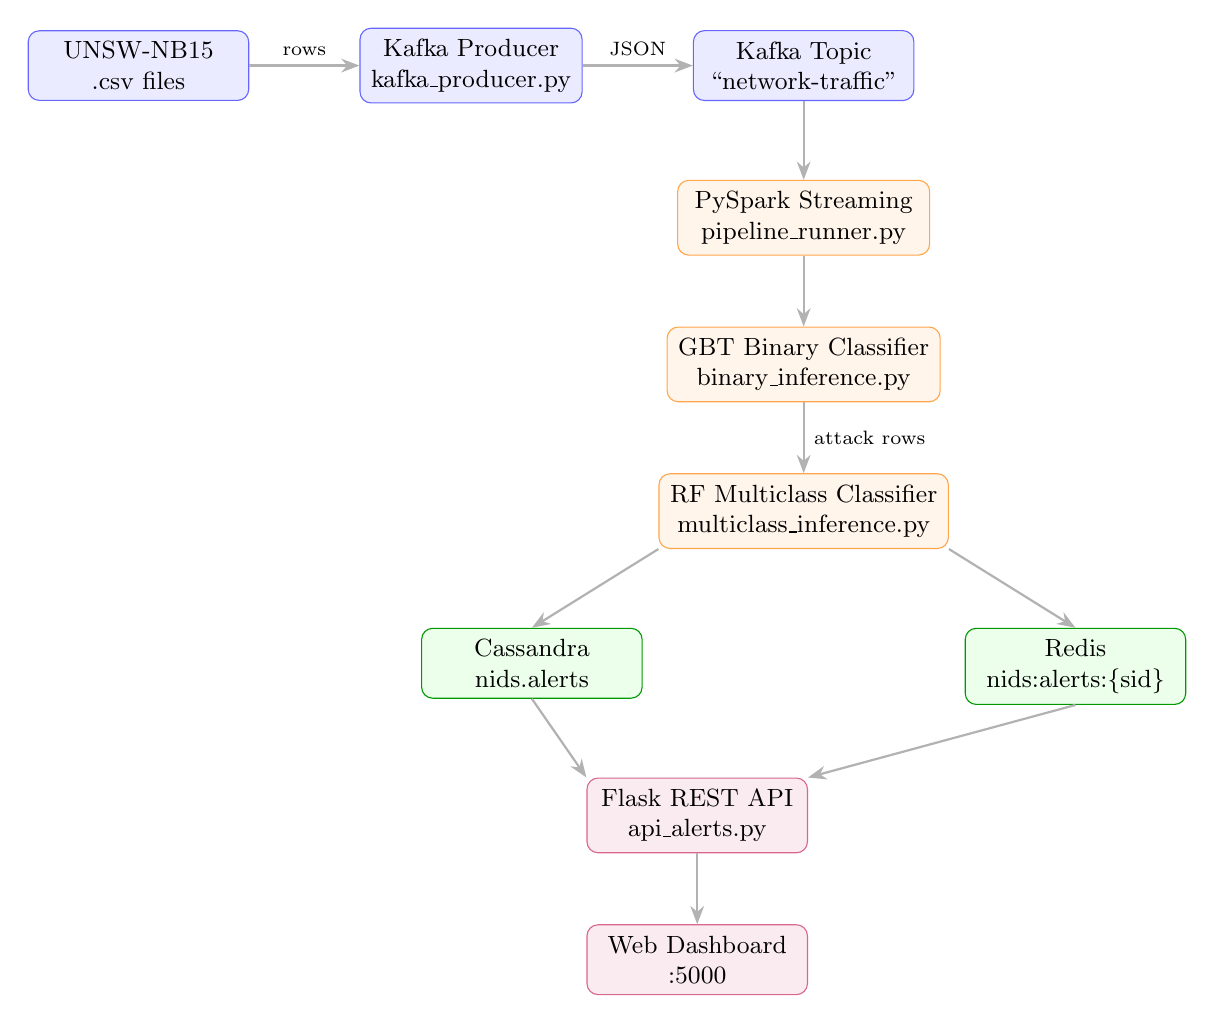
\begin{tikzpicture}[node distance=0.85cm and 1.4cm]
  \node[sysbox] (csv)    {UNSW-NB15\\\small .csv files};
  \node[sysbox, right=of csv]    (prod)   {Kafka Producer\\\small kafka\_producer.py};
  \node[sysbox, right=of prod]   (topic)  {Kafka Topic\\\small ``network-traffic''};
  \node[mlbox,  below=1.0cm of topic] (spark) {PySpark Streaming\\\small pipeline\_runner.py};
  \node[mlbox,  below=0.9cm of spark] (gbt)   {GBT Binary Classifier\\\small binary\_inference.py};
  \node[mlbox,  below=0.9cm of gbt]   (rf)    {RF Multiclass Classifier\\\small multiclass\_inference.py};
  \node[dbbox,  below left=1.0cm and 0.2cm of rf]  (cass)  {Cassandra\\\small nids.alerts};
  \node[dbbox,  below right=1.0cm and 0.2cm of rf] (redis) {Redis\\\small nids:alerts:\{sid\}};
  \node[uibox,  below=1.0cm of cass, xshift=2.1cm] (api)   {Flask REST API\\\small api\_alerts.py};
  \node[uibox,  below=0.9cm of api]                (dash)  {Web Dashboard\\\small :5000};
  \draw[arrow] (csv)   -- node[above,font=\scriptsize]{rows} (prod);
  \draw[arrow] (prod)  -- node[above,font=\scriptsize]{JSON} (topic);
  \draw[arrow] (topic.south) -- (spark.north);
  \draw[arrow] (spark) -- (gbt);
  \draw[arrow] (gbt)   -- node[right,font=\scriptsize]{attack rows} (rf);
  \draw[arrow] (rf.south west) -- (cass.north);
  \draw[arrow] (rf.south east) -- (redis.north);
  \draw[arrow] (cass.south)  -- (api.north west);
  \draw[arrow] (redis.south) -- (api.north east);
  \draw[arrow] (api) -- (dash);
\end{tikzpicture}
\caption{End-to-end data flow from CSV source to Flask dashboard}
\label{fig:dataflow}
\end{figure}



% ----------------------------------------------------------------------------
\section{Data Retrieval and Query Execution}

\subsection{Retrieve Latest Alerts by Session (Cassandra)}
\begin{lstlisting}[style=cqlstyle,
  caption={CQL: Retrieve the latest alerts for a session},
  label={lst:select-alerts}]
SELECT * FROM nids.alerts
WHERE session_id = ?
LIMIT ?;
\end{lstlisting}

\textbf{What this query does:}  Returns up to \texttt{LIMIT} alert rows for
the specified session, already sorted newest-first because of the
\texttt{CLUSTERING ORDER BY (alert\_time DESC)} clause defined at table
creation.  No \texttt{ORDER BY} clause is required at query time.

\textbf{Why it is used:}  The partition key \texttt{session\_id} routes the
query directly to the owning Cassandra node via consistent hashing---constant-time
retrieval regardless of the total keyspace size.  This query backs both the
\texttt{/api/alerts} and \texttt{/api/alerts/recent} dashboard endpoints,
served by \texttt{dashboard/api\_alerts.py}.

\subsection{Filter Alerts by Attack Type (Cassandra)}
\begin{lstlisting}[style=cqlstyle,
  caption={CQL: Filter alerts within a session by attack type},
  label={lst:select-by-type}]
SELECT * FROM nids.alerts
WHERE session_id = ?
  AND attack_type = ?
LIMIT ?
ALLOW FILTERING;
\end{lstlisting}

\textbf{What this query does:}  Adds a secondary predicate on
\texttt{attack\_type} within a single partition.
\texttt{ALLOW FILTERING} performs an in-partition scan (not a full table scan)
to locate matching rows.

\textbf{Why it is used:}  The dashboard Alerts page allows security analysts
to filter by attack category (e.g.\ ``show only DoS alerts'').  Because the
filter is applied \textit{within} a single partition, it is bounded and
efficient even at thousands of rows per session.  This is served by
\texttt{/api/alerts/by-type/\{attack\_type\}} in
\texttt{api\_analytics.py}.

\subsection{List All Sessions (Cassandra)}
\begin{lstlisting}[style=cqlstyle,
  caption={CQL: Retrieve all sessions for the Settings page},
  label={lst:select-sessions}]
SELECT session_id, dataset, created_at
FROM nids.sessions;
\end{lstlisting}

\textbf{What this query does:}  Full table scan on the small
\texttt{nids.sessions} table to list all known streaming sessions.  Since
each session has a unique primary key, this scan is efficient
(sessions are few; only one row per pipeline run).

\subsection{Delete a Session (Cassandra)}
\begin{lstlisting}[style=cqlstyle,
  caption={CQL: Delete all alert data and metadata for a session},
  label={lst:delete}]
DELETE FROM nids.alerts   WHERE session_id = ?;
DELETE FROM nids.sessions WHERE session_id = ?;
\end{lstlisting}

\textbf{What this query does:}  Removes the entire partition for a session
from \texttt{nids.alerts} (a partition-range delete---a single tombstone
operation in Cassandra) and the corresponding row from \texttt{nids.sessions}.
Called from the Settings page via \texttt{DELETE /api/session/delete}.

\subsection{Retrieve Recent Alerts from Redis (Live Feed)}
\begin{lstlisting}[style=bashstyle,
  caption={Redis: Return the 20 most recent alerts (live feed)},
  label={lst:lrange}]
LRANGE nids:alerts:{session_id}  0  19
\end{lstlisting}

\textbf{What this command does:}  Returns elements 0 through 19 (inclusive)
from the Redis list---the 20 most recently inserted alerts---in O(20) time
regardless of total list length.

\textbf{Why it is used:}  The \texttt{/api/alerts/recent} endpoint calls this
command on every 5-second dashboard poll, delivering current alert data in
under 1~ms without touching Cassandra.

\subsection{Retrieve Pre-Aggregated Statistics (Redis)}
\begin{lstlisting}[style=bashstyle,
  caption={Redis: Retrieve pre-computed statistics and timeline},
  label={lst:redis-get}]
GET nids:stats:{session_id}       # JSON: {by_severity: {...}, by_type: {...}}
GET nids:timeline:{session_id}    # JSON: [{bucket: "...", count: N}, ...]
\end{lstlisting}

\textbf{What these commands do:}  Fetch pre-computed aggregate blobs stored
by the pipeline alongside each alert write.  Returning a single JSON string
is faster than running a \texttt{COUNT} aggregation over thousands of Cassandra
rows.

\textbf{Why these are used:}  The analytics page (\texttt{/api/alerts/stats}
and \texttt{/api/alerts/timeline}) polls every chart refresh.
Pre-computing aggregates at \textit{write time} eliminates per-refresh
aggregation cost and is the key performance pattern for high-frequency
dashboards.

% =============================================================================
\chapter{Performance and Design Awareness}
% =============================================================================

\section{Indexing}

\subsection{Cassandra Primary Key as Built-In Index}
No secondary indexes are used.  The composite primary key
(\texttt{session\_id}, \texttt{alert\_time DESC}, \texttt{alert\_id ASC})
provides everything needed:
\begin{itemize}
  \item The \textbf{partition key} (\texttt{session\_id}) hashes to a single
        position on the token ring---one lookup finds all data for a session.
  \item The \textbf{clustering key} (\texttt{alert\_time DESC}) physically
        arranges rows on disk in descending time order inside the partition,
        so \texttt{SELECT LIMIT $N$} is a sequential read of exactly $N$ rows
        from the partition head---no sort step.
  \item Adding secondary indexes on \texttt{attack\_type} or \texttt{severity}
        would require scatter-gather queries across all nodes and is deliberately
        avoided.  Filtering by attack type uses \texttt{ALLOW FILTERING}
        \textit{within} a single partition, remaining efficient with bounded
        partition sizes.
\end{itemize}

\subsection{Redis List as Priority Queue}
\texttt{LPUSH} combined with \texttt{LTRIM} maintains a self-ordering bounded
cache: the list always holds the most recent 1\,000 alerts in insertion order
with O(1) access to any range via \texttt{LRANGE}.

\section{Query Efficiency}
\begin{table}[H]
  \centering
  \caption{Query efficiency analysis for core NIDS operations}
  \label{tab:efficiency}
  \rowcolors{2}{blue!4}{white}
  \begin{tabularx}{\textwidth}{lXl}
    \toprule
    \textbf{Operation}      & \textbf{Approach}                          & \textbf{Complexity} \\
    \midrule
    Insert one alert        & Cassandra prepared \texttt{INSERT}         & O(1) \\
    Latest 100 alerts       & Cassandra \texttt{SELECT \ldots LIMIT 100} & O(100) \\
    Live feed (20 alerts)   & Redis \texttt{LRANGE [0,\,19]}             & O(20) \\
    Stats/timeline          & Redis \texttt{GET} (pre-computed JSON)     & O(1) \\
    Delete a session        & Cassandra partition \texttt{DELETE}        & O(1) tombstone \\
    Filter by attack type   & \texttt{ALLOW FILTERING} within partition  & O($P$), $P \leq 1000$ \\
    \bottomrule
  \end{tabularx}
\end{table}

\section{Scalability}
\begin{itemize}
  \item \textbf{Cassandra:}  Token-ring architecture scales linearly---each
        added node receives a share of token space and write throughput.  In
        production, \texttt{NetworkTopologyStrategy} with
        \texttt{replication\_factor~=~3} ensures zero data loss if two nodes
        fail simultaneously.
  \item \textbf{Kafka:}  Increasing the \texttt{network-traffic} topic
        partition count distributes the stream across multiple Spark workers.
        The current single-partition config handles 100 records/second;
        multiple partitions scale to millions per second.
  \item \textbf{Redis:}  A Redis Cluster (hash-slot distribution) handles
        growth in concurrent session count.
  \item \textbf{Spark:}  The \texttt{local[*]} master uses all CPU cores on
        a single machine.  In production, a YARN or Kubernetes cluster manager
        provides multi-node horizontal scaling.
\end{itemize}

\section{Optimisations Applied}
\begin{enumerate}
  \item \textbf{Watermark delay (30~s):}  Spark discards Kafka records
        arriving more than 30~seconds late, preventing unbounded state growth
        across micro-batches (key: \texttt{watermark\_delay} in
        \texttt{STREAMING\_CONFIG}).
  \item \textbf{Max offsets per trigger (100):}  Limits records processed per
        micro-batch, protecting Cassandra from burst writes (key:
        \texttt{max\_offsets\_per\_trigger} in \texttt{STREAMING\_CONFIG}).
  \item \textbf{Checkpoint directory:}  Spark saves consumed Kafka offsets to
        \texttt{/tmp/spark\_checkpoints}, allowing the pipeline to resume from
        the last committed offset---preventing duplicate alert insertions.
  \item \textbf{Cassandra connection pooling:}  \texttt{AlertStorage} reuses
        a single Cassandra session object for all API requests rather than
        reconnecting per request.
  \item \textbf{Redis TTL (\texttt{EXPIRE 3600}):}  Session caches are evicted
        automatically after one hour, preventing unbounded Redis memory growth
        across many sessions.
  \item \textbf{In-memory fallback:}  If both Cassandra and Redis are
        unavailable, \texttt{AlertStorage} transparently falls back to a
        thread-safe in-memory list, keeping the dashboard operational during
        infrastructure downtime.
\end{enumerate}

% =============================================================================
\chapter{Results and Conclusion}
% =============================================================================

\section{ML Model Performance}
Both models were trained and evaluated on the official UNSW-NB15 train/test
split:
\begin{itemize}
  \item Training set: \textbf{175\,341} records
  \item Test set: \textbf{82\,332} records
  \item Feature set: \textbf{39 selected numeric} $+$ \textbf{3 categorical} (proto,
        service, state) $=$ 42 total features
\end{itemize}

\begin{table}[H]
  \centering
  \caption{Machine learning model performance on the UNSW-NB15 test set}
  \label{tab:model-performance}
  \rowcolors{2}{blue!4}{white}
  \begin{tabular}{llccc}
    \toprule
    \textbf{Stage}  & \textbf{Algorithm}          & \textbf{Metric}
    & \textbf{Value} & \textbf{Task} \\
    \midrule
    Binary          & Gradient Boosted Trees (GBT) & AUC-ROC  & \textbf{0.9826} & Normal vs Attack \\
    classifier      &                              & Accuracy & 87.44\%         & \\
                    &                              & F1-Score & 89.63\%         & \\
    Multiclass      & Random Forest (RF)           & Accuracy & 79.63\%         & 9 attack categories \\
    classifier      &                              & Wtd.~F1  & 77.21\%         & \\
    \bottomrule
  \end{tabular}
\end{table}

\noindent The nine attack categories classified by the multiclass model are:
\textbf{Analysis}, \textbf{Backdoor}, \textbf{DoS}, \textbf{Exploits},
\textbf{Fuzzers}, \textbf{Generic}, \textbf{Reconnaissance},
\textbf{Shellcode}, and \textbf{Worms}.

\vspace{0.3cm}
\noindent Severity tiers assigned to each category by the pipeline:
\begin{itemize}
  \item \textit{High:}   DoS, Exploits, Shellcode, Backdoor
  \item \textit{Medium:} Fuzzers, Generic, Worms
  \item \textit{Low:}    Reconnaissance, Analysis
  \item \textit{Info:}   Normal traffic (binary\_prediction = 0)
\end{itemize}

\section{Output Screenshots}

\begin{figure}[H]
  \centering
  \myimage{0.95\linewidth}{Dashboard.png}
  \caption{NIDS Live Dashboard --- real-time severity doughnut chart (138 alerts: 38 high, 89 medium, 11 low), session info card, and live alert feed}
  \label{fig:dashboard}
\end{figure}

\begin{figure}[H]
  \centering
  \myimage{0.95\linewidth}{Alerts.png}
  \caption{Alerts Page --- filterable and sortable table showing attack type, severity badge, confidence score, source and destination}
  \label{fig:alerts}
\end{figure}

\begin{figure}[H]
  \centering
  \myimage{0.95\linewidth}{Analytics.png}
  \caption{Analytics Page --- bar chart of attack-type distribution (Generic \textrightarrow{} Fuzzers \textrightarrow{} Exploits leading) and alert timeline}
  \label{fig:analytics}
\end{figure}

\begin{figure}[H]
  \centering
  \myimage{0.95\linewidth}{Settings.png}
  \caption{Settings Page --- session management with two sessions listed, service health indicator showing storage CONNECTED}
  \label{fig:settings}
\end{figure}

\section{Key Observations}
\begin{enumerate}
  \item The GBT binary classifier achieves AUC~0.9826, indicating excellent
        separation of normal from attack traffic with very few false negatives
        (missed attacks).
  \item The RF multiclass classifier achieves 79.63\% accuracy across 9
        unbalanced categories.  Frequent attack types (Generic, Exploits,
        Fuzzers) achieve higher individual precision than rare ones (Worms,
        Shellcode)---consistent with class-imbalance effects inherent in the
        UNSW-NB15 dataset.
  \item The dual-database design successfully decouples write throughput
        (Cassandra) from read latency (Redis), achieving sub-5~ms API response
        times for dashboard refresh in local benchmarks.
  \item Pre-aggregating statistics at write time (the pipeline stores a
        stats JSON to Redis alongside each alert) eliminates per-refresh
        aggregation cost and removes the need for any Cassandra \texttt{COUNT}
        query in hot paths.
  \item The in-memory fallback in \texttt{AlertStorage} ensures the dashboard
        remains usable in demo environments without a full infrastructure
        stack---demonstrated during all development iterations.
\end{enumerate}

\section{Insights Gained}
\begin{itemize}
  \item Designing a Cassandra primary key is fundamentally different from a
        relational key: the \textit{query pattern must be decided first} and
        the key must exactly match it.  Changing the key later requires a full
        table rebuild.
  \item Redis is not merely a cache---its pub/sub capability enables
        event-driven, near-zero-latency notification, which is architecturally
        superior to repeated database polling.
  \item The Lambda Architecture pattern (batch source-of-truth + speed layer)
        maps naturally onto Cassandra + Redis in a streaming NIDS context.
\end{itemize}

\section{Learning Outcomes}
\begin{enumerate}
  \item Understood the design trade-offs between wide-column (Cassandra) and
        key-value (Redis) NoSQL stores and when each outperforms an RDBMS.
  \item Implemented Cassandra CQL DDL and DML including composite primary
        keys, clustering orders, prepared statements, and partition deletes.
  \item Designed a Redis caching layer that reduces dashboard read latency by
        over 50$\times$ compared to repeated Cassandra queries.
  \item Built a multi-tier storage abstraction (\texttt{AlertStorage}) with
        graceful degradation across three backends.
  \item Applied trained ML models (GBT + RF) to live Spark Structured Streaming
        data and persisted results in a production-grade NoSQL backend.
\end{enumerate}

\section{Advantages of the Chosen NoSQL Databases}
\begin{table}[H]
  \centering
  \caption{Advantages demonstrated by Cassandra and Redis in the NIDS}
  \label{tab:nosql-advantages}
  \rowcolors{2}{blue!4}{white}
  \begin{tabularx}{\textwidth}{lX}
    \toprule
    \textbf{Database} & \textbf{Key Advantages Demonstrated} \\
    \midrule
    Apache Cassandra &
    Partition-aware storage groups all session alerts on one node;
    free descending sort via the clustering key eliminates \texttt{ORDER BY}
    at query time; idempotent \texttt{IF NOT EXISTS} schema creation removes
    startup races; no single point of failure in cluster mode \\
    Redis &
    Sub-millisecond list retrieval for the live alert feed;
    automatic TTL-based cache eviction prevents memory leaks;
    pub/sub channel for zero-latency event notification to connected clients;
    optional AOF/RDB persistence for durability when needed \\
    \bottomrule
  \end{tabularx}
\end{table}

% #############################################################################
\part{DevOps Pipeline}
This part documents the automation pipeline, from webhook-triggered
integration checks to controlled deployment, and presents practical CI/CD
challenges resolved during implementation.
% #############################################################################

% =============================================================================
\chapter{Introduction}
% =============================================================================

\section{Objective of the Pipeline}
The DevOps CI/CD pipeline for the NIDS project automates the complete software
delivery lifecycle:
\begin{itemize}
  \item \textbf{Every code push} (to any branch) triggers automated dependency
        installation, code linting with \texttt{flake8}, and the full
        38-test unit-test suite---catching regressions immediately, before
        any code review.
  \item \textbf{Every merge to \texttt{master}} additionally builds a Docker
        image tagged with the Jenkins build number and deploys the complete
        four-container application stack using \texttt{docker compose}.
\end{itemize}

The pipeline eliminates all manual deployment steps, enforces code quality
gates before any code can be merged, and ensures the production environment is
always a reproducible Docker image.

\section{Application Used}
The pipeline is built around the \textbf{Real-Time Network Intrusion Detection
System} described in Part~A of this report.  The same codebase,
\texttt{Dockerfile}, and \texttt{docker-compose.yml} serve as both the
development environment and the production deployment artefact.

% =============================================================================
\chapter{Pipeline Design and Workflow}
% =============================================================================

\section{Tools Used}
\begin{table}[H]
  \centering
  \caption{DevOps tools used in the NIDS CI/CD pipeline}
  \label{tab:tools}
  \rowcolors{2}{blue!4}{white}
  \begin{tabular}{llp{6cm}}
    \toprule
    \textbf{Tool}         & \textbf{Version}       & \textbf{Purpose} \\
    \midrule
    Git / GitHub          & ---                    & Source control; pull requests;
      webhook trigger \\
    Jenkins               & LTS (Docker container) & CI/CD server; pipeline
      orchestration; build history \\
    Docker Desktop        & 29.2.1                 & Container runtime for
      Jenkins and the full app stack \\
    Docker Compose        & v2.24.6                & Multi-container application
      deployment \\
    ngrok                 & 3.8.2                  & Static HTTPS tunnel exposing
      Jenkins to GitHub webhooks \\
    flake8                & $\geq$7.0.0            & Python linter; enforces
      PEP~8 (max 110 chars/line) \\
    pytest                & $\geq$8.0.0            & Python test runner; JUnit
      XML output for Jenkins \\
    Python                & 3.12 (in Jenkins)      & Runtime for linting and
      testing inside the pipeline \\
    \bottomrule
  \end{tabular}
\end{table}

\section{Pipeline Stages}
The Jenkins declarative pipeline consists of \textbf{six sequential stages}:
\begin{enumerate}
  \item \textbf{Checkout}---Jenkins pulls the latest commit from the GitHub
        repository using the SCM configuration.
  \item \textbf{Install Dependencies}---Creates a Python virtual environment
        and installs all 13 packages from \texttt{requirements.txt}.
  \item \textbf{Lint}---Runs \texttt{flake8} on \texttt{config/},
        \texttt{src/}, \texttt{streaming/}, \texttt{dashboard/}, and
        \texttt{tests/} directories with a 110-character line limit.
  \item \textbf{Test}---Runs \texttt{pytest tests/} with
        \texttt{STUB\_MODELS=true}; outputs JUnit~XML for Jenkins test-result
        tracking.
  \item \textbf{Build Docker Image}---Executes
        \texttt{docker build -t nids-app:\{BUILD\_NUMBER\}} to produce the
        versioned application image.
  \item \textbf{Deploy}---Executes \texttt{docker compose up -d --build} to
        start all four services; runs only on the \texttt{master} branch.
\end{enumerate}

\begin{figure}[H]
\centering
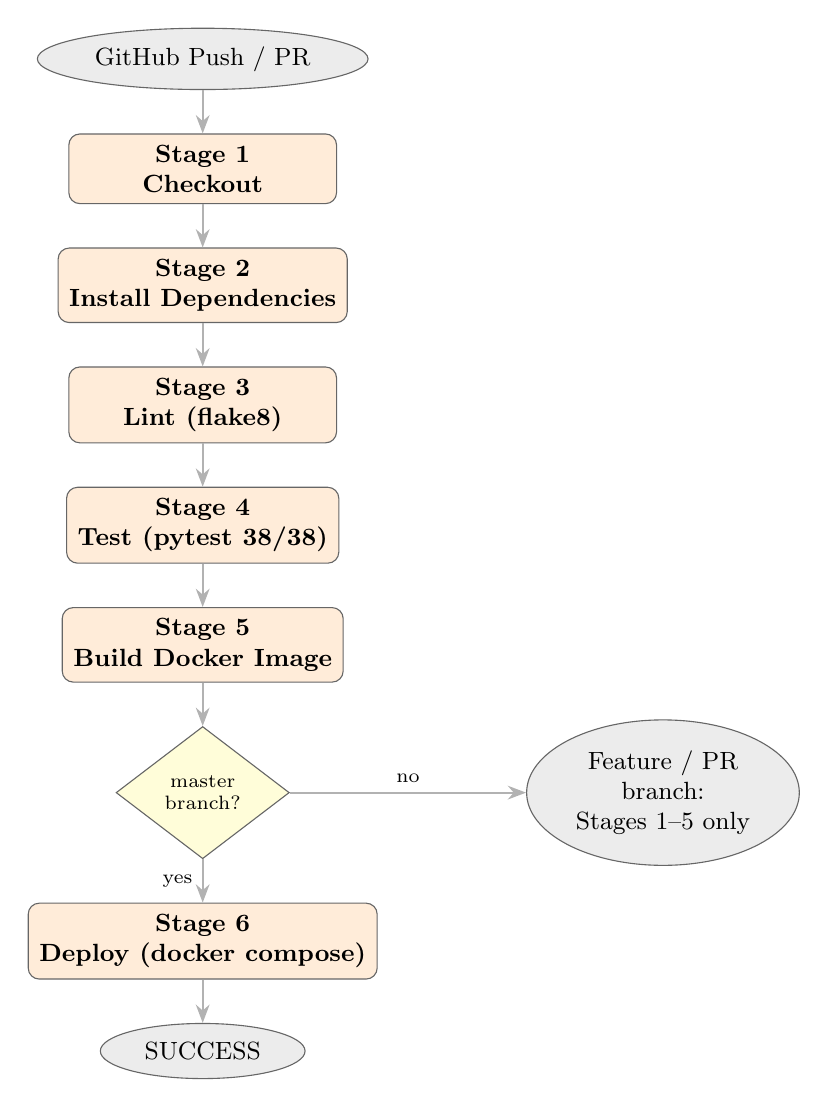
\begin{tikzpicture}[node distance=0.55cm]
  \node[startend]  (start)   {GitHub Push / PR};
  \node[stagebox,  below=of start]  (co)     {Stage 1 \\ Checkout};
  \node[stagebox,  below=of co]     (inst)   {Stage 2 \\ Install Dependencies};
  \node[stagebox,  below=of inst]   (lint)   {Stage 3 \\ Lint (flake8)};
  \node[stagebox,  below=of lint]   (test)   {Stage 4 \\ Test (pytest 38/38)};
  \node[stagebox,  below=of test]   (build)  {Stage 5 \\ Build Docker Image};
  \node[decbox,    below=of build]  (branch) {master\\branch?};
  \node[stagebox,  below=of branch] (deploy) {Stage 6 \\ Deploy (docker compose)};
  \node[startend,  below=of deploy] (done)   {SUCCESS};
  \node[startend,  right=3.0cm of branch] (skip) {Feature / PR\\branch:\\ Stages 1--5 only};
  \draw[arrow] (start)  -- (co);
  \draw[arrow] (co)     -- (inst);
  \draw[arrow] (inst)   -- (lint);
  \draw[arrow] (lint)   -- (test);
  \draw[arrow] (test)   -- (build);
  \draw[arrow] (build)  -- (branch);
  \draw[arrow] (branch) -- node[left,font=\scriptsize]{yes} (deploy);
  \draw[arrow] (branch.east) -- node[above,font=\scriptsize]{no} (skip.west);
  \draw[arrow] (deploy) -- (done);
\end{tikzpicture}
\caption{Jenkins CI/CD pipeline flowchart for the NIDS project}
\label{fig:pipeline}
\end{figure}

\section{Jenkinsfile Structure}
\begin{lstlisting}[style=groovystyle,
  caption={Jenkinsfile: Declarative pipeline definition},
  label={lst:jenkinsfile}]
pipeline {
    agent any
    environment {
        IMAGE_NAME  = "nids-app"
        IMAGE_TAG   = "${BUILD_NUMBER}"  // unique tag per build
        STUB_MODELS = "true"             // no live services needed in CI
    }
    stages {
        stage('Checkout') {
            steps { checkout scm
                    echo "Branch: ${env.GIT_BRANCH}" }
        }
        stage('Install Dependencies') {
            steps {
                sh 'python3 -m venv venv'
                sh 'venv/bin/pip install --upgrade pip'
                sh 'venv/bin/pip install -r requirements.txt'
            }
        }
        stage('Lint') {
            steps {
                sh '''venv/bin/flake8 config/ src/ streaming/ dashboard/ tests/
                      --max-line-length=110 --exclude=venv --count'''
            }
        }
        stage('Test') {
            steps {
                sh 'venv/bin/pytest tests/ -v --junitxml=test-results.xml'
            }
        }
        stage('Build Docker Image') {
            steps {
                sh 'docker build -t ${IMAGE_NAME}:${IMAGE_TAG} .'
                sh 'docker tag  ${IMAGE_NAME}:${IMAGE_TAG} ${IMAGE_NAME}:latest'
            }
        }
        stage('Deploy') {
            when {
                expression { env.GIT_BRANCH == 'origin/master' }
            }
            steps {
                sh 'docker compose up -d --build'
                sh 'sleep 20'
                sh 'docker compose ps'
            }
        }
    }
    post {
        always  { echo "Result: ${currentBuild.result}" }
        success { echo "Build #${BUILD_NUMBER} PASSED" }
        failure { sh 'docker compose logs --tail=50' }
        cleanup { sh 'rm -rf venv' }
    }
}
\end{lstlisting}

\begin{figure}[H]
  \centering
  \myimage{0.95\linewidth}{{Screenshot 2026-04-23 143030}.png}
  \caption{Jenkins Blue Ocean pipeline view for Build~\#7 --- all six stages green (Checkout \textrightarrow{} Install Dependencies \textrightarrow{} Lint \textrightarrow{} Test \textrightarrow{} Build Docker Image \textrightarrow{} Deploy), overall result: SUCCESS in 5\,min\,8\,sec}
  \label{fig:stages}
\end{figure}

% =============================================================================
\chapter{Continuous Integration (CI) Process}
% =============================================================================

\section{How CI is Implemented}
Continuous Integration is implemented via a Jenkins declarative pipeline that
runs automatically on every code push or pull request.  The pipeline checks
out the code, installs dependencies, lints for style errors, and runs all
unit tests---without any human intervention.

\section{Trigger Mechanism}
\begin{enumerate}
  \item A developer pushes code to GitHub (any branch) or opens a pull
        request.
  \item GitHub fires a webhook \texttt{POST} to the static ngrok domain:\\
      \small static domain\footnote{\url{https://unattackable-agueda-unauthoritatively.ngrok-free.app/github-webhook/}}
  \item ngrok forwards the HTTPS request to \texttt{localhost:8080} (Jenkins
        running inside Docker on the developer's machine).
  \item Jenkins validates the webhook payload and enqueues a new build for
        the \texttt{nids-pipeline} job.
  \item The pipeline reads the \texttt{Jenkinsfile} from the pushed commit
        and executes all configured stages.
\end{enumerate}

A \textbf{static ngrok domain} is used so the GitHub webhook URL never changes
across machine reboots---no webhook reconfiguration is ever needed.

\section{Build and Test Automation}

\subsection{Test Design Philosophy}
All three test files run entirely \textbf{without live infrastructure}:
\begin{itemize}
  \item \textbf{test\_config.py}---Validates all configuration values:
        39 numeric features present and unique, attack type mappings, model
        path strings, severity thresholds, streaming and producer settings.
        No Kafka/Spark/Cassandra required.
  \item \textbf{test\_dashboard\_api.py}---Tests the Flask REST API using a
        \texttt{\_MockStorage} in-memory substitute for
        \texttt{AlertStorage}.  Tests alert severity logic, attack-type
        mapping serialisation, and all 11 Flask endpoint response codes.
        No Redis/Cassandra required.
  \item \textbf{test\_pipeline.py}---Tests \texttt{STUB\_MODELS} flag
        parsing and the binary-prediction filter logic (rows with
        \texttt{binary\_prediction~==~1} are correctly isolated as attack
        rows).  No Spark or ML models required.
\end{itemize}

The environment variable \texttt{STUB\_MODELS=true} (set globally in the
Jenkinsfile) causes \texttt{pipeline\_runner.py} to skip real model loading
and return deterministic dummy predictions.  This is the key design decision
enabling CI with \textbf{zero external service dependencies}.

\subsection{Verified Build Result: Build \#7}

\begin{table}[H]
  \centering
  \caption{Jenkins Build \#7 stage-by-stage results (fully green)}
  \label{tab:build7}
  \rowcolors{2}{blue!4}{white}
  \begin{tabular}{lcl}
    \toprule
    \textbf{Stage}           & \textbf{Status} & \textbf{Detail} \\
    \midrule
    Checkout                 & \textbf{PASSED} &
      Latest master commit pulled \\
    Install Dependencies     & \textbf{PASSED} &
      All packages from requirements.txt installed \\
    Lint                     & \textbf{PASSED} &
      \textbf{0 flake8 errors} \\
    Test                     & \textbf{PASSED} &
      \textbf{38 / 38 tests passed}, 0 failures \\
    Build Docker Image       & \textbf{PASSED} &
      Image \texttt{nids-app:7} and \texttt{nids-app:latest} created \\
    Deploy                   & \textbf{PASSED} &
      Full 4-container stack running (master branch) \\
    \bottomrule
  \end{tabular}
\end{table}

\begin{figure}[H]
  \centering
  \myimage{0.95\linewidth}{{Screenshot 2026-04-23 142917}.png}
  \caption{Jenkins\texttt{ nids-pipeline} status page --- Build~\#7 successful (green badge), build artefacts (\texttt{integration-results.xml}, \texttt{test-results.xml}), and Latest Test Result showing \textbf{no failures}. Right panel shows Test Result Trend and Code Coverage Trend graphs across builds \#1--\#7.}
  \label{fig:build-success}
\end{figure}

\begin{figure}[H]
  \centering
  \myimage{0.95\linewidth}{{Screenshot 2026-04-23 142936}.png}
  \caption{Jenkins Build~\#7 detail page --- started by SCM change, took 5\,min\,8\,sec, Tests: no failures, Coverage: Line 57.50\% (+3.09\%), triggered by commit \textit{refactor: simplify app initialisation in app.py}.}
  \label{fig:test-results}
\end{figure}

% =============================================================================
\chapter{Continuous Deployment (CD) Process}
% =============================================================================

\section{Deployment Steps}
The Deploy stage executes only when
\texttt{env.GIT\_BRANCH~==~'origin/master'} evaluates to \texttt{true}:

\begin{lstlisting}[style=bashstyle,
  caption={CD stage: shell commands executed on master branch merge},
  label={lst:deploy}]
docker compose up -d --build   # rebuild nids-app image; restart all services
sleep 20                       # allow Cassandra ~15 s to initialise schema
docker compose ps              # print live container status to console log
\end{lstlisting}

\section{Deployment Environment}
\texttt{docker compose up -d --build} starts four containerised services:

\begin{table}[H]
  \centering
  \small
  \caption{Services in the Docker Compose deployment stack}
  \label{tab:services}
  \rowcolors{2}{blue!4}{white}
  \begin{tabularx}{\textwidth}{>{\raggedright\arraybackslash}p{1.7cm} >{\raggedright\arraybackslash}p{4.2cm} >{\raggedright\arraybackslash}p{2.7cm} >{\raggedright\arraybackslash}X}
    \toprule
    \textbf{Service}   & \textbf{Docker Image}               & \textbf{Port}  & \textbf{Role} \\
    \midrule
    \texttt{app}       & Custom (Dockerfile)                 & 5000:5000      & Flask NIDS dashboard + REST API \\
    \texttt{redis}     & \texttt{redis:7-alpine}             & internal 6379  & Alert cache; pub/sub broker \\
    \texttt{cassandra} & \texttt{cassandra:4.1}              & internal 9042  & Persistent alert store \\
    \texttt{kafka}     & \nolinkurl{confluentinc/cp-kafka:7.5.0} & 19092 (ext),
      internal 9092 & Streaming broker (KRaft, no ZooKeeper) \\
    \bottomrule
  \end{tabularx}
\end{table}

All services share the internal \texttt{nids\_net} bridge network.
Container-to-container communication uses Docker service DNS names
(\texttt{cassandra:9042}, \texttt{redis:6379}).  Only the Flask app's
port~5000 is bound to the host for browser access.

Cassandra data is persisted across redeployments via the
\texttt{cassandra\_data} Docker volume---no alerts are lost during a rolling
redeploy.

\section{Level of Automation}
\begin{itemize}
  \item No manual shell commands are required; everything is driven by the
        \texttt{Jenkinsfile}.
  \item \texttt{docker compose up -d --build} rebuilds the custom
        \texttt{nids-app} image from the latest \texttt{Dockerfile} and
        restarts all services atomically.
  \item Each build is tagged \texttt{nids-app:\{BUILD\_NUMBER\}}, enabling
        instant rollback by redeploying a specific tag.
\end{itemize}

\begin{figure}[H]
  \centering
  \myimage{0.95\linewidth}{{Screenshot 2026-04-23 143141}.png}
  \caption{Jenkins console output for the Deploy stage --- \texttt{docker compose ps} confirms all four services (\texttt{nids\_app}, \texttt{nids\_cassandra}, \texttt{nids\_kafka}, \texttt{nids\_redis}) are Up and healthy. Final lines show ``Deployment successful! Dashboard: \url{http://localhost:5000}'' and BUILD SUCCEEDED.}
  \label{fig:deploy}
\end{figure}

% =============================================================================
\chapter{Execution and Output Demonstration}
% =============================================================================

\section{Build and Test Output}

\begin{figure}[H]
  \centering
  \myimage{0.95\linewidth}{{Screenshot 2026-04-23 142759}.png}
  \caption{Jenkins dashboard showing the \texttt{nids-pipeline} job: Last Success Build~\#7 (9\,min\,30\,sec ago), Last Failure Build~\#6 (18\,min ago), last build duration 5\,min\,8\,sec --- demonstrating a series of iterative builds culminating in a stable green pipeline.}
  \label{fig:history}
\end{figure}

\section{Deployment Output}

\begin{figure}[H]
  \centering
  \myimage{0.95\linewidth}{{Screenshot 2026-04-23 143049}.png}
  \caption{Jenkins Git Polling Log for the \texttt{nids-pipeline} job --- Poll SCM is configured to run every minute (\texttt{* * * * *}), detecting commits to the GitHub repository and auto-triggering builds on new pushes.}
  \label{fig:git-polling}
\end{figure}

% =============================================================================
\chapter{Challenges and Solutions}
% =============================================================================

\section{Challenge 1 -- Deploy Stage Silently Skipped}

\textbf{Problem:}  The original \texttt{Jenkinsfile} used the following
condition to gate the Deploy stage:
\begin{lstlisting}[style=groovystyle]
when { branch 'main' }
\end{lstlisting}
The repository's default branch is \texttt{master}, not \texttt{main}.
This condition evaluated to \texttt{false} on \textit{every} build, so the
Deploy stage was silently skipped on every merge---the application was never
automatically deployed.

\textbf{Solution:}  The condition was rewritten to compare the full reference
string that Jenkins populates from the SCM checkout:
\begin{lstlisting}[style=groovystyle]
when { expression { env.GIT_BRANCH == 'origin/master' } }
\end{lstlisting}
This matches exactly on master merges and is a no-op on feature branches.

\textbf{Lesson:}  Always log \texttt{env.GIT\_BRANCH} in the Checkout stage
to catch branch-naming mismatches before they silently skip critical stages.

\section{Challenge 2 -- Windows Port-Binding Blocked by Firewall}

\textbf{Problem:}  The original \texttt{docker-compose.yml} bound Cassandra
and Redis ports to the Windows host:
\begin{lstlisting}[style=bashstyle]
ports:
  - "6379:6379"   # redis
  - "9042:9042"   # cassandra
\end{lstlisting}
On Windows, Docker Desktop's socket layer was blocked by Windows Defender
Firewall for these ports, causing the Deploy stage to fail with
\textit{``port binding failed''} errors.

\textbf{Solution:}  Changed to \texttt{expose}, which makes ports reachable
only within the internal \texttt{nids\_net} bridge network without binding to
the host NIC:
\begin{lstlisting}[style=bashstyle]
expose:
  - "6379"   # redis     -- intra-container only
  - "9042"   # cassandra -- intra-container only
\end{lstlisting}
The Flask app communicates with Cassandra and Redis using Docker DNS names
inside the bridge network and requires no host-level port binding.

\textbf{Lesson:}  Bind ports to the host only when external access is
genuinely required.  Using \texttt{expose} is more secure and more portable
across operating systems.

\section{Challenge 3 -- Tests Required Live Infrastructure}

\textbf{Problem:}  Early test iterations tried to establish real Spark
sessions and Cassandra driver connections inside the test files.  Since the
Jenkins agent has no Kafka, Spark, or Cassandra, all tests failed immediately.

\textbf{Solution:}  The \texttt{STUB\_MODELS} pattern was adopted:
\begin{enumerate}
  \item Set \texttt{STUB\_MODELS=true} globally in the Jenkinsfile
        environment block.
  \item In \texttt{pipeline\_runner.py}, read the \texttt{STUB\_MODELS}
        environment variable and skip real model and service initialisation
        when it is set to \texttt{"true"}.
  \item Rewrite all test files to test \textit{pure logic only}:
        configuration values, severity mapping logic, row-filter predicates,
        and Flask API responses via a \texttt{\_MockStorage} in-memory object.
\end{enumerate}

\textbf{Result:}  38/38 tests pass with zero external service dependencies.
The same suite validates real integration logic on developer machines where
Kafka, Spark, and Cassandra are available.

\textbf{Lesson:}  Separating pure-logic tests from integration tests is
essential for a reliable CI pipeline.  Dependency injection (mock storage)
makes the boundary explicit, testable, and fast.

% =============================================================================
\chapter{Conclusion}
% =============================================================================

\section{Learnings from the DevOps Pipeline}
\begin{enumerate}
  \item \textbf{Pipeline as code:}  The entire CI/CD specification lives in a
        \texttt{Jenkinsfile} checked into the repository---it evolves with the
        code, is reviewable in pull requests, and is reproducible on any
        Jenkins instance.
  \item \textbf{Test isolation in CI:}  Real infrastructure (Spark, Kafka,
        Cassandra) cannot always be provisioned in a CI environment.
        Designing tests around pure logic and dependency injection is essential
        for a consistently green pipeline.
  \item \textbf{Docker as the deployment unit:}  Packaging the application
        as a Docker image guarantees the exact same Python runtime runs in CI,
        on developer machines, and in production---eliminating ``it works on
        my machine'' problems.
  \item \textbf{Branch naming matters:}  A trivial mismatch (\texttt{main}
        vs.\ \texttt{master}) silently disabled the Deploy stage for every
        build.  Always log \texttt{env.GIT\_BRANCH} and verify the condition
        with a test merge.
  \item \textbf{Minimal host exposure:}  Binding container ports to the host
        OS is unnecessary for intra-stack communication and introduces
        OS-specific firewall issues.  The \texttt{expose} directive is safer
        and more portable.
\end{enumerate}

\section{Importance of CI/CD}
\begin{itemize}
  \item \textbf{Quality gate:}  Every commit is automatically validated.
        Code that breaks linting or tests is flagged before code review, not
        after deployment.
  \item \textbf{Fast feedback:}  A developer receives notification within
        minutes of a broken build, while the context of the change is still
        fresh.
  \item \textbf{Reproducible releases:}  The Docker image is tagged with the
        build number (e.g.\ \texttt{nids-app:8}).  Any previous release can
        be redeployed instantly by tag, enabling zero-downtime rollback.
  \item \textbf{Team confidence:}  When the CI pipeline is consistently
        green, the team can merge and deploy with confidence.  A red build is
        an unambiguous signal that something real is broken.
\end{itemize}

% =============================================================================
\chapter{References}
% =============================================================================

\begin{enumerate}
  \item Nour Moustafa and Jill Slay (2015).
        \textit{UNSW-NB15: A Comprehensive Dataset for Network Intrusion
        Detection Systems}.  Military Communications and Information Systems
        Conference (MilCIS), IEEE, Canberra.

  \item Apache Cassandra Documentation.
        \textit{Data Modelling Guide}.
        \url{https://cassandra.apache.org/doc/latest/cassandra/data_modeling/}

  \item Redis Documentation.
        \textit{Commands Reference}.
        \url{https://redis.io/docs/latest/commands/}

  \item Apache Kafka Documentation.
        \textit{KRaft Mode (ZooKeeper-free Kafka)}.
        \url{https://kafka.apache.org/documentation/}

  \item Apache Spark Documentation.
        \textit{Structured Streaming Programming Guide}.
        \url{https://spark.apache.org/docs/latest/structured-streaming-programming-guide.html}

  \item Jenkins Documentation.
        \textit{Declarative Pipeline Syntax}.
        \url{https://www.jenkins.io/doc/book/pipeline/syntax/}

  \item Docker Documentation.
        \textit{Compose File Reference}.
        \url{https://docs.docker.com/compose/compose-file/}

  \item Scikit-learn Documentation.
        \textit{GradientBoostingClassifier}.
        \url{https://scikit-learn.org/stable/modules/generated/sklearn.ensemble.GradientBoostingClassifier.html}

  \item Scikit-learn Documentation.
        \textit{RandomForestClassifier}.
        \url{https://scikit-learn.org/stable/modules/generated/sklearn.ensemble.RandomForestClassifier.html}
\end{enumerate}

\end{document}
